\documentclass{article}
\usepackage[
backend=biber,
style=alphabetic,
sorting=ynt
]{biblatex}

\usepackage{geometry}
\geometry{letterpaper, left=20mm, right=20mm, top=20mm, bottom=20mm}
 
\usepackage[acronym]{glossaries}

\usepackage{optidef}
\addbibresource{mybibliography.bib}

\makeglossaries

\newglossaryentry{LM} {name=LM,
    description={Language model. E.g., GPT-3, PaLM}
}
\newglossaryentry{RM}{name=RM,
    description={Retrieval model. E.g., Classical lexical IR, ColBERTv2}}

\title{Literature Review \\
       \large Open domain QA for financial enterprise}
\author{Sasi Kanth Ala}
\date{March 2023}

\begin{document}
\maketitle

\section{Introduction}
 Knowledge intensive question answering (QA) is challenging to implement in a finance enterprise due to regulations around privacy and confidentiality of financial information. Some of the techniques used in state of the art trained closed QA systems may not provide the required control over who can access what information and when. Classical (or neural) information retrieval (IR) systems can easily be modified to support information access controls. For example Elasticsearch workplace search Confluence connector can import access-control lists and filter out information based on user authorization at search time. Recently open-domain question answering (OpenQA) systems which use a language model (LM) and a retrieval model (RM) are becoming competitive with ClosedQA systems. QA systems with information access controls can be implemented with a frozen LM and RM with access controls. Classical IR systems are also good at updating inverted indices so that the information can be kept up to date. There are many techniques for tweaking relevance like boosting of documents based on metadata (document update time), page rank or from learning to rank. 

Single-hop OpenQA may not provide much extra benefit when compared to plain IR, but multi-hop open-domain QA will give significant boost to user's efficiency.

\section{Summaries of articles}
  \subsection{DEMONSTRATE-SEARCH-PREDICT \cite{https://doi.org/10.48550/arxiv.2212.14024}}
Using retrieval models (RM) to search for relevant information and then using in-context learning of large language models (LM) to summarize it has become a powerful technique for knowledge intensive tasks such as complex question answering systems. Previous work combined these into simple retrieve-then-read pipelines which uses passages retrieved by RM and inserted into LM to generate answers. This paper introduces a framework called Demonstrate-Search-Predict (DSP) that relies on passing information between the LM and RM in sophisticated ways. DSP is a framework whose primitives can be used to write a high level programs which create demonstrations, search for passages and make predictions. This paper evaluates DSP programs for multi-hop open domain question answering.

LM have issues with hallucinations where they produce grammatically correct unsupported or incorrect answers. Simple retrieve and read pipeline has trouble with complex questions where a single passage may not have the complete answer. DSP programs can decompose the problem use multiple hops to retrieve passages and provide the correct answer.

DSP framework has composable primitives which can be used to bootstrap training examples (demonstrate), gather information for corpus (search) and then predict (predict). 

The authors evaluate the DSP programs using frozen LM GPT-3.5 and frozen RM ColBERTv2. They evaluate 3 different NLP tasks - open-domain QA, multi-hop QA and conversational QA. The data sets selected are SQuAD, multi-hop HotPotQA and QReCC dataset respectively to evaluate the above tasks. The DSP programs deliver 37-120\%,8-39\% and 80-290\% against plain LM, standard retrieve-then-read pipeline, and self-ask pipeline respectively. The reported numbers are for validation set.

The authors argue for a task aware strategies for pipelines using DSP primitives for high performing NLP systems.

This paper is interesting as the components of the system talk to each other in natural language and uses frozen LM and RM which they argue will allow for broadened participation in AI system development.

  \subsection{Answering Complex Open-Domain Questions with Multi-Hop Dense Retrieval \cite{https://doi.org/10.48550/arxiv.2009.12756}}
Authors of this paper propose a multi-hop dense retrieval approach for complex open-domain QA. This approach does not use corpus specific information like hyperlinks or entity markers and work on unstructured corpus. 

This approach uses dense passage retrieval method instead of classical IR which uses lexical matching and may fail to capture semantics. Dense passage retrieval uses vector representations of query and passages and relies on maximum inner-product search (MIPS). Simpler questions where the answer is fully contained in a passage can be answered by one interaction RM but complex questions where the answer is spread across multiple passages need multiple interactions with RM. 

Main issue with multi-hop approach is that the search space grows exponentially with every hop. Previous works tackle this by using entity or hyperlink structure to create a document graph and the problem becomes what is the best way to traverse this graph. These strategies will not work with unstructured corpus. In this paper authors propose a way to use encode the query and the retrieved documents as a query vector and retrieve the next relevant document using MIPS methods. 

The authors simple concatenate the query and previous retrieval results and use query encoder to product dense representation of query for next retrieval. Instead of using separately parameterized encoder for question and passages they use a shared RoBERTa-base encoder for both query and passage encoding. Specifically they use layer normalization over the start token's representation from RoBERTa to get the final query/passage vectors.

For evaluation the authors use HotpotQA and multi-evidence subset of FEVER. They show significant improvements retrieval performance when compared to TF-IDF, TF-IDF + Linked, DrKIT and Entity Linking. 

Authors also did a retrieval error analysis of question categories (bridged questions, comparison questions) in HotpotQA. They found that comparison questions are easier as both entities needed for retrieval are present in the question. From analysing comparison question errors they postulate that using retrieval method which uses both term and dense index might improve performance on bridge questions.

They also found that using explicit question decomposition which helps with TF-IDF retriever does not improve performance in dense retriever. They postulate that the strong pre-trained encoders can effectively learn to select necessary information from multi-hop question at each step.

  \subsection{MEASURING AND NARROWING THE COMPOSITIONALITY GAP IN LANGUAGE MODELS \cite{https://doi.org/10.48550/arxiv.2210.03350}}
This paper investigates the gap between how well a LM can answer compositional reasoning task vs. how well it can answer the sub-problems involved in the compositional reasoning task. This gap is called compositionality gap. This gap gives up some idea on how well a LM can reason. The authors show that in GPT-3 family of models the compositionalty gap does not decrease with the model size. This suggests that the large models memorize and recall than reason. The authors also demonstrate how chain of thought prompting narrows the compositionality gap by reasoning explicitly. They present a new model called self-ask which improves the chain of thought. This self-ask will allow plugging in search engine by intercepting LMs output and can be used for open domain complex QA.

Authors generated a automatically generated 2-hop dataset called Compositional Celebrities (CC) with 8.6k questions. An example: "Who won the Master's Tournament the year Justin Bieber was born?". This dataset is used to investigate the compositionality gap. They show that in large number of cases LMs fail to compose two facts which were observed separately during pretraining. 

Figure \ref{fig:self-ask} shows a example of how self-ask prompts work. An RM can intercept these intermediate questions and can insert answers which can be used as a multi-hop open domain question answering system.

\begin{figure}[htp]
    \centering
    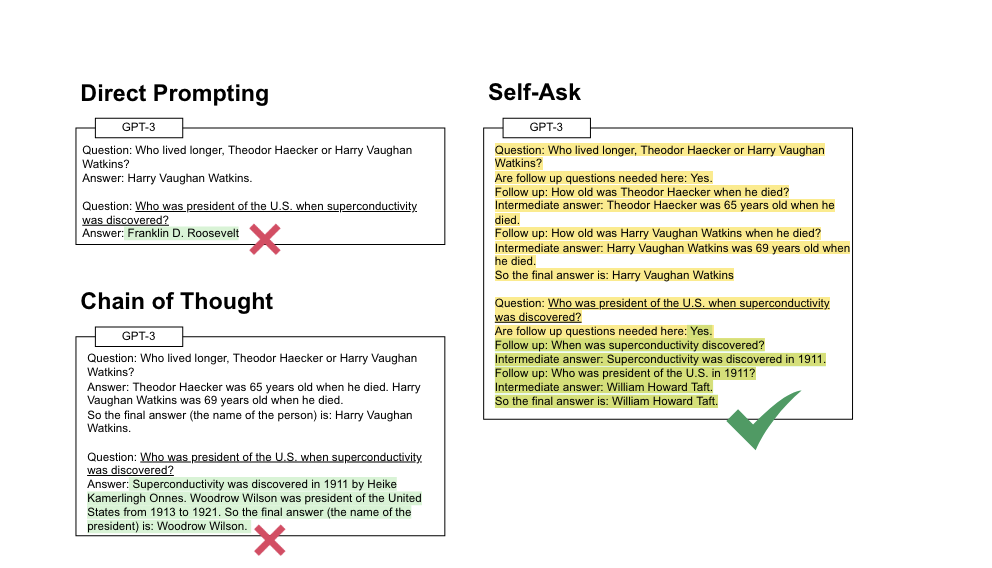
\includegraphics[width=6cm]{self-ask-prompts.png}
    \caption{direct prompting vs. chain of though vs. self-ask prompts\cite{https://doi.org/10.48550/arxiv.2210.03350}}
    \label{fig:self-ask}
\end{figure}

  \subsection{RARR: Researching and Revising What Language Models Say, Using Language Models \cite{https://doi.org/10.48550/arxiv.2210.08726}}
Currently LMs excel in many tasks like question answering, few shot learning and dialog. But they have problem of generating misleading or wrong (hallucinations) predictions. LMs can't do attributions to external evidence. The authors or this paper propose a way to retrofit attribution using research and revision (RARR). The system automatically finds attribution from out of any text generation model and edits the output to fix unsupported context while preserving the original output as much as possible. This model is reverse of other common technique of retrieving relevant passages and then prompting LMs with this passage to generate predictions. 

To measure the quality of their system they measure the quality of revised text along attribution and preservation dimensions. Attribution is how much of the revised text is attributed to the evidence retrieved. Preservation is how much of the revised text preserves the aspect of original. In development they used a NLI model to approximate human judgements about attribution. And they used a metric based on Levenshtein distance to measure how much the original and the revised text differ.

Authors use in-context learning of LM to develop many components of RARR. They used PALM as their LM. RARR goes through 4 phases: query generation, retrieval, agreement and edit. In question generation phase they prompt LM with six hundred demonstrations of CQGen (comprehensive question generation). They also run the model three times and take a union of questions for diversity and coverage of questions. In retrieval phase the generated queries are submitted to google and top 5 results are selected and snippets extracted. The snippets are ranked using a relevance model and first J are selected for each query. Agreement model is also based on few shot promoting which will predict if the original statement is in agreement with the article retrieved. Depending on the output of agreement check there may be a edit phase. In the edit phase the LM is again used to correct the original output. Figure \ref{fig:RARR-prompts} show example prompts. 

\begin{figure}[htp]
    \centering
    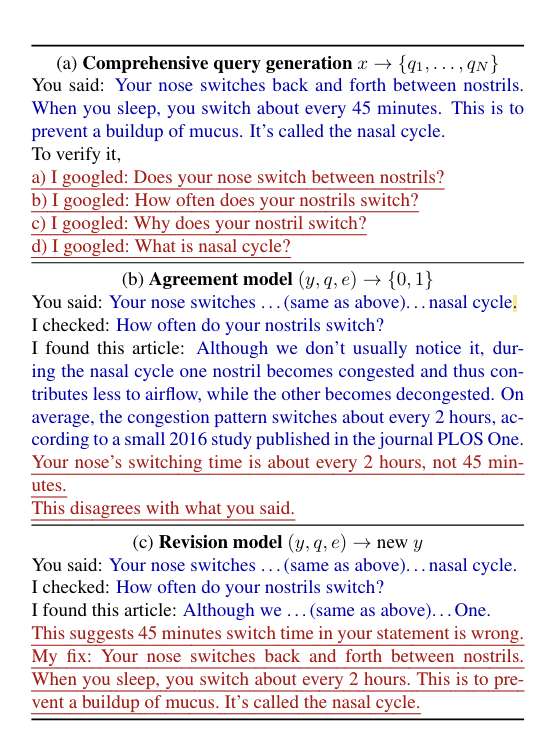
\includegraphics[width=6cm]{RARR-prompts.png}
    \caption{RARR: Example prompts (summary) \cite{https://doi.org/10.48550/arxiv.2210.08726}}
    \label{fig:RARR-prompts}
\end{figure}

The authors found that the size of the LM (PaLM 540B vs. PaLM 62B) has large effect on the performance of RARR. They postulate that increases in LM's scale will improve RARR performance.

  \subsection{ColBERTv2: Effective and Efficient Retrieval via Lightweight Late Interaction \cite{https://doi.org/10.48550/arxiv.2112.01488}}
This paper deals with improving space efficiency of ColBERT a late interaction neural retriever. ColBERT independently encodes query and passages using BERT and employs a cheap later interaction step that models the similarity between query and passages. ColBERT is competitive with BERT based baseline while having four orders of magnitude query latency. Authors of this paper are able to reduce space utlization of ColBERT by 6-10x. 

ColBERTv2 uses residual representation based on evidence that ColBERT vectors cluster into regions. First ColBERTv2 find a set of centroids and encodes each vectors as index of the centroid close to it and quantized residual. At search time the approximate vector is recovered using the centroid and the residual vector. ColBERTv2 is able to compress vectors to 20 or 36 bytes when compared to 256 bytes for ColBERT. 

\section{Compare and contrast}
Large LM with in-context learning opened up a new way of implementing NLP systems. Self-ask, DSP and RARR all extensively use prompting of a LM in their implementation. Self-ask\cite{https://doi.org/10.48550/arxiv.2210.03350} prompts a LM to split a complex question into component questions which can be answered by looking up in a RM. It is able to beat direct prompting, chain of though and retrieve-then-read pipelines in multi-hop QA.
DSP\cite{https://doi.org/10.48550/arxiv.2212.14024} provides a generic framework where knowledge-based talks can be solved by complex interactions between LM and RM. Self-ask can be implemented using a simple DSP program. DSP can be used to write more sophisticated pipelines where DSP program manages control flow and thus more robust than self-ask where LM manages control flow. MDR (multi-hop dense retriever)\cite{https://doi.org/10.48550/arxiv.2009.12756} is different from the previous papers in that it does not use LM in directing searches. It encodes the question and passages retrieved from previous step to search for next passages in a dense retriever.    

RARR\cite{https://doi.org/10.48550/arxiv.2210.08726} uses a reverse generate and fix a reverse strategy of retrieve-and-read. In RARR LM is used to generate text and RM is used for finding support for the statements and fixing them. RARR also extensively use prompting of LMs for generating fact checking questions and fixing of original text based on answers from RM.

\section{Future work}
DSP framework allows for implementing various high level programs for knowledge intensive tasks. It will be interesting to investigate what strategies work best for a OpenQA in particular domain (for e.g, finance). It will also be interesting to investigate what additional primitives and building blocks can be added to make this framework usable in finance domain. For e.g having access to a database with financial data, or access to a calculator.    
\medskip

\printbibliography
\end{document}
